\let\negmedspace\undefined
\let\negthickspace\undefined
\documentclass[journal]{IEEEtran}
\usepackage[a5paper, margin=10mm, onecolumn]{geometry}
%\usepackage{lmodern} % Ensure lmodern is loaded for pdflatex
\usepackage{tfrupee} % Include tfrupee package

\setlength{\headheight}{1cm} % Set the height of the header box
\setlength{\headsep}{0mm}     % Set the distance between the header box and the top of the text

\usepackage{gvv-book}
\usepackage{gvv}
\usepackage{cite}
\usepackage{amsmath,amssymb,amsfonts,amsthm}
\usepackage{algorithmic}
\usepackage{graphicx}
\usepackage{textcomp}
\usepackage{xcolor}
\usepackage{txfonts}
\usepackage{listings}
\usepackage{enumitem}
\usepackage{mathtools}
\usepackage{gensymb}
\usepackage{comment}
\usepackage[breaklinks=true]{hyperref}
\usepackage{tkz-euclide} 
\usepackage{listings}
% \usepackage{gvv}                                        
\def\inputGnumericTable{}                                 
\usepackage[latin1]{inputenc}                                
\usepackage{color}                                            
\usepackage{array}                                            
\usepackage{longtable}                                       
\usepackage{calc}                                             
\usepackage{multirow}                                         
\usepackage{hhline}                                           
\usepackage{ifthen}                                           
\usepackage{lscape}
\begin{document}

\bibliographystyle{IEEEtran}
\vspace{3cm}

\title{4.10.13}
\author{EE25BTECH11012-BEERAM MADHURI}
% \maketitle
% \newpage
% \bigskip
{\let\newpage\relax\maketitle}

\renewcommand{\thefigure}{\theenumi}
\renewcommand{\thetable}{\theenumi}
\setlength{\intextsep}{10pt} % Space between text and floats


\numberwithin{equation}{enumi}
\numberwithin{figure}{enumi}
\renewcommand{\thetable}{\theenumi}
\textbf{Question}:\\Find the equation of the plane passing through the line of intersection of the planes
$\vec{r} \cdot (\hat{i} + \hat{j} + \hat{k}) = 1$ and $\vec{r} \cdot (2\hat{i} + 3\hat{j} - \hat{k}) + 4 = 0$ and parallel to the $X$ axis.\\
\textbf{Solution:}\\
let P1 and P2 be the plane equations whose normals are:
\begin{table}[h!]
    \centering
    \begin{tabular}{|c|c|}
\hline
\textbf{Name} & \textbf{Value} \\
\hline
Circle & $\vec{x}^\top\vec{x} - a^2 = 0$ \\
\hline
Line & $\vec{x} = \myvec{\tfrac{a}{\sqrt{2}} \\ 0} + \kappa\myvec{0 \\ 1}$ \\
\hline
\end{tabular}

    \caption{4.10.13}
    \label{table 4.10.13}
\end{table}

Given equations of planes are:-
\begin{align}
P_1: \quad \vec{r}^\top \begin{pmatrix} 1 \\ 1 \\ 1 \end{pmatrix} = 1\\
P_2: \quad \vec{r}^\top \begin{pmatrix} 2 \\ 3 \\ -4 \end{pmatrix} = -4
\end{align}
expressing the plane equations in matrix form:-
\begin{align}
\begin{bmatrix}1 & 1 & 1 & | & 1 \\2 & 3 & -4 & | & -4\end{bmatrix}
\end{align}
Using row reductions:
\begin{align}
R_2 \rightarrow R_2 - 2R_1\\
\begin{bmatrix}1 & 1 & 1 & | & 1 \\0 & 1 & -3 & | & -6\end{bmatrix}\\
\therefore \text{equation of planes:}\\
\vec{r}^\top \begin{pmatrix} 1 \\ 1 \\ 1 \end{pmatrix} = 1\\
\vec{r}^\top \begin{pmatrix} 0 \\ 1 \\ -3 \end{pmatrix} = -6
\end{align}
Solving the equations to find the line of intersection of planes\\
\begin{align}
\vec{r}(\lambda) = \begin{pmatrix}0 \\-\frac{3}{4} \\\frac{7}{6}\end{pmatrix} + \lambda \begin{pmatrix}1 \\-3/4 \\-1/6\end{pmatrix}
\end{align}\\
\text{normal to plane is orthogonal to the line and x-axis}
\begin{align}
\vec{n}^\top \vec{e}_1 = 0\\
\vec{n}^\top \vec{n}_1 = 0
\end{align}
\begin{align*}
where,  
\end{align*}
\begin{align}
\vec{e}_1 = \begin{pmatrix} 1 \\ 0 \\ 0 \end{pmatrix}\\ \vec{n}_1 = \begin{pmatrix} 1 \\ -3/4 \\ -1/6 \end{pmatrix}
\end{align}
\text{Solving using row reductions:-}
\begin{align}
\begin{bmatrix}1 & 0 & 0 & | & 0 \\4 & -3 & -1 & | & 0\end{bmatrix}
\end{align}
\begin{align}
R_2 \rightarrow R_2 - 4R_1
\end{align}
\begin{align}
\begin{bmatrix}1 & 0 & 0 & | & 0 \\0 & -3 & -1 & | & 0\end{bmatrix}
\end{align}
\text{plane equation using normal and a point on the line:}
\begin{align}
\vec{n}^\top (\vec{r} - \vec{r}_0) = 0\\
\vec{r}_0 = \begin{pmatrix} 0 \\ -3/4 \\ -7/4 \end{pmatrix}\\
\vec{n} = \begin{pmatrix}0 \\1 \\-3\end{pmatrix}\\
\vec{r} = \begin{pmatrix}x \\y \\z\end{pmatrix}
\end{align}
Hence, equation of the plane is: $y - 3z + 6 = 0$ 

\begin{figure}[H]
    \centering
    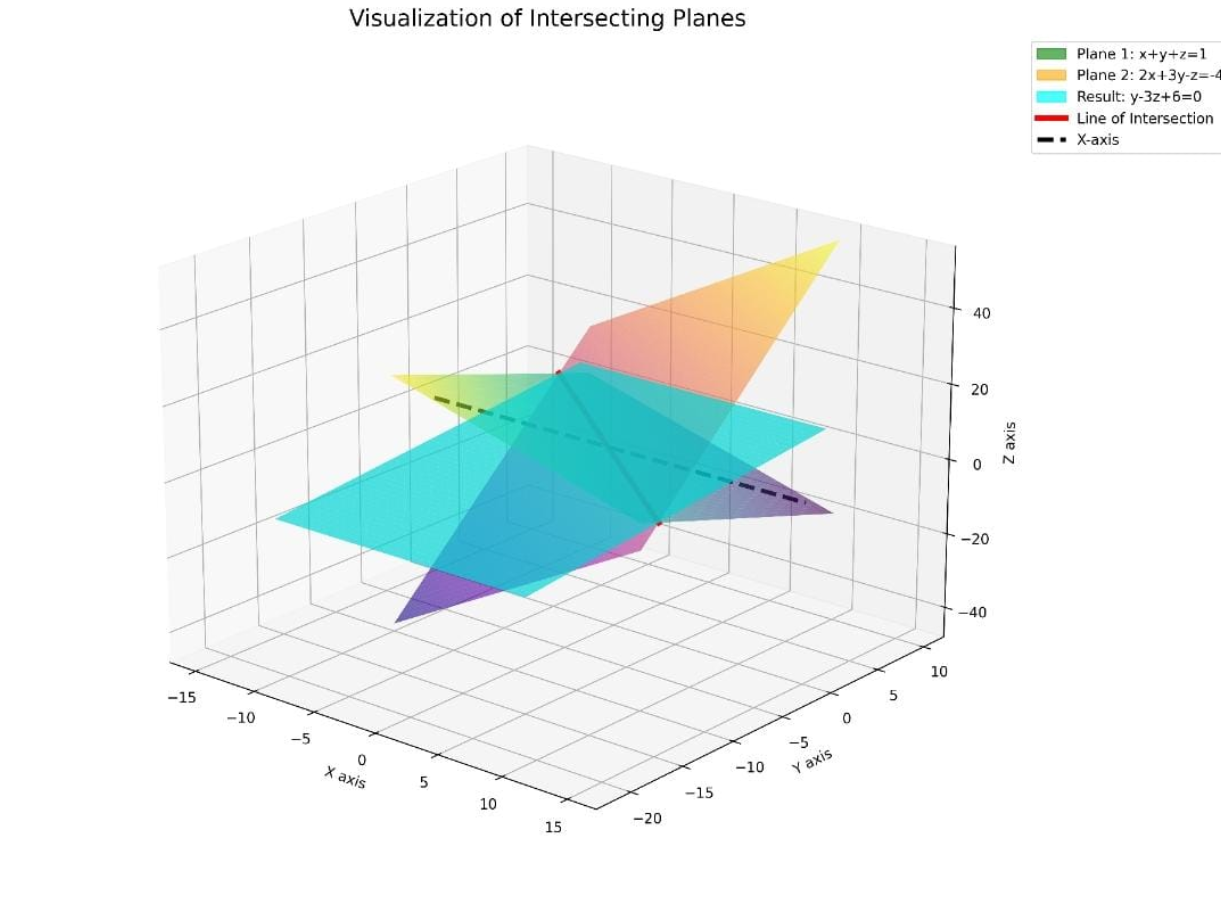
\includegraphics[width=0.85\columnwidth]{figs/graph.png}
    \caption{4.10.13}
    \label{fig:4.10.13}
\end{figure}


\end{document}


